\documentclass{article}

\usepackage{titlesec}
\usepackage{amsmath}
\usepackage{mathtools}
\usepackage{enumitem}
\usepackage{listings}
\usepackage{float}
\usepackage[utf8]{inputenc}
\usepackage{xcolor}
\usepackage{graphicx}
\usepackage{subcaption}
\usepackage{tikz}
\usepackage{textcomp}

\usetikzlibrary{quotes,angles}

\definecolor{codegreen}{rgb}{0,0.6,0}
\definecolor{codegray}{rgb}{0.5,0.5,0.5}
\definecolor{codepurple}{rgb}{0.58,0,0.82}
\definecolor{backcolour}{rgb}{0.95,0.95,0.92}

\lstdefinestyle{mystyle}{
    backgroundcolor=\color{backcolour},   
    basicstyle=\ttfamily\footnotesize,
    breakatwhitespace=false,
    breaklines=true,
    captionpos=b,
    keepspaces=true,
    numbers=left,
    numbersep=5pt,
    showspaces=false,
    showstringspaces=false,
    showtabs=false,
    tabsize=2
}

\graphicspath{ {./assets} }

\lstset{style=mystyle}

\author{William B. Sørensen}
\title{MST125 TMA01}
\begin{document}
\maketitle

\section{Question 1}

\tableofcontents

\subsection{a}

\begin{center}
	\textbf {MST125 TMA 01 Question 1}

	William Bjørn Sørensen, I220215X

	\LaTeX
\end{center}

\subsection{b}

\begin{enumerate}
	\item The distance between $\mathrm A(x_1,~y_1)$ and $\mathrm B(x_2,~y_2)$ is given by
	      \begin{align*}
		      \mathrm {AB} & = \sqrt{{(x_2-x_1)}^2 + {(y_2-y_1)}^2} \mathrm.
	      \end{align*}
	      Hence the distance between $\mathrm A (-3,~1)$ and $\mathrm B (2,~-2)$ is
	      \begin{align*}
		      \mathrm {AB} & = \sqrt{{(2-(-3))}^2 + {(-1-1)}^2} \\
		                   & = \sqrt {5^2 + (-3)^2}             \\
		                   & = \sqrt {34}\mathrm .
	      \end{align*}

	\item The gradient $m$ of the line through $(x_1,~y_1)$ and $(x_2,~y_2)$ is given by
	      \begin{align*}
		      m = \frac {y_2 - y_1} {x_2 - x_1} \mathrm .
	      \end{align*}
	      Hence the gradient of the line through $(-3,~1)$ and $(2,~-2)$ is
	      \begin{align*}
		      m = \frac {-2-1} {2-(-3)} & = -\frac 35\mathrm .
	      \end{align*}

	\item The gradient of the line is $-\frac 35$. Hence $\tan \alpha = - \frac 35$.
	      Let $\phi$ be the acute angle that the line makes with the nagative direction of the $x$-axis. Then
	      \begin{align*}
		      \tan \phi & = \frac 35 \mathrm ,
	      \end{align*}
	      so
	      \begin{align*}
		      \phi & = \tan^{-1} \Big( \frac 35 \Big) = 0.540\dots\mathrm .
	      \end{align*}
	      Hence
	      \begin{align*}
		      \alpha & = \pi - 0.540\dots = 2.601 \dots \mathrm .
	      \end{align*}
	      Therefore the angle $\alpha$ is $2.60$ radiants (to 2 d.p.).
\end{enumerate}

\subsection{c}

I intend to typeset my TMA through the fact that I believe the programatic power of \LaTeX is a great advantage. Through MST125 I have even started using \LaTeX over Markdown (with mathjax) for school assignemts now.

Using \LaTeX in my daily school work leads me to a much DRYer (don't repeat yourself) documents where all my associate code can be refrenced with great accuracy without suffering from complecated compilation scripts.

I have also configured a Vim integration so I can use my primary editor for TMAs.

\section{Question 2}

\begin{enumerate}[label=(\alph*)]
	\item Find the least residue of $64^7$ modulo $15$.
	      \begin{align*}
		      64^7 & \equiv x \mod {15} \\
		      4^7  & \equiv x \mod {15}
	      \end{align*}
	      We observe $4^2 \equiv 1 \mod {15}$.
	      \begin{align*}
		      4^1  & \equiv x \mod {15} \\
		      64^7 & \equiv 4 \mod {15} \\
	      \end{align*}
\end{enumerate}

\section{Question 3}

\subsection{a}

\subsubsection{i}

We find the $\gcd$ using Euler's algorithm. These variable names come from CAS tool I wrote in Rust for Unit3.

$$\begin{matrix}
		a  &   & q &        & b  &   & r \\
		90 & = & 5 & \times & 17 & + & 5 \\
		17 & = & 3 & \times & 5  & + & 2 \\
		5  & = & 2 & \times & 2  & + & 1 \\
		2  & = & 2 & \times & 1  & + & 0
	\end{matrix}$$

We reshape for substitution

$$\begin{matrix}
		\textcircled 5 & = & \textcircled {90} & - & 5 & \times & \textcircled {17} \\
		\textcircled 2 & = & \textcircled {17} & - & 3 & \times & \textcircled 5    \\
		\textcircled 1 & = & \textcircled 5    & - & 2 & \times & \textcircled 2
	\end{matrix}$$
And then conduct said substitution
\begin{align*}
	a \times \textcircled {17} + b \times \textcircled {90} & = \textcircled 1                                                                                                                               \\
	                                                        & = \textcircled 5     -  2  \times \textcircled 2                                                                                               \\
	                                                        & = (\textcircled {90}  -  5  \times  \textcircled {17})-  2  \times \textcircled 2                                                              \\
	                                                        & = (\textcircled {90}  -  5  \times  \textcircled {17})-  2  \times (\textcircled {17} - 3 \times \textcircled 5)                               \\
	                                                        & = (\textcircled {90} - 5 \times \textcircled {17}) - 2 \times (\textcircled {17} - 3 \times (\textcircled {90} - 5  \times \textcircled {17})) \\
	                                                        & = 7 \times \textcircled {90} - 37  \times \textcircled {17}
\end{align*}

Then we find the least residual of $-37$ and deduce that the multiplicative inverse of $17 \mod 90$ is $53$.

This means the solution to $17 x \equiv 9 \mod 90$ is $x \equiv 53 \times 9 \equiv 477 \equiv 27 \mod 90$.

\subsubsection{ii}

We begin by simplifying the congruence.

$$\begin{matrix}
		a & x & \equiv & b  & \mod & n  \\
		9 & x & \equiv & 12 & \mod & 90 \\
		3 & x & \equiv & 4  & \mod & 30
	\end{matrix}$$

As we can see here $\gcd (3,30) \ne 1$ and $3 \not|\;4$ so the congruence is unsolvable.

\subsubsection{iii}


We begin by simplifying the congruence.

$$\begin{matrix}
		a  & x & \equiv & b  & \mod & n  \\
		27 & x & \equiv & 72 & \mod & 90 \\
		3  & x & \equiv & 8  & \mod & 10 \\
	\end{matrix}$$

This is small enougth for a brute force attack but for clarities sake I will not do this.

We can see they are coprime. Hence we can skip Euler's algo.

\begin{align*}
	\textcircled{10}a + \textcircled 3b & = 1                                           \\
	                                    & = \textcircled {10} - 3 \times \textcircled 3
\end{align*}

We find least residual and multiply with $8$. So $x \equiv -3 \times 8 \equiv 7 \times 8 \equiv 56 \equiv 6 \mod 10$.

\subsection{b}

\subsubsection{i}

$$7 \times 15 \equiv 105 \equiv 4 \times 26 + 1 \equiv 1 \mod 26$$

\subsubsection{ii}

$$\begin{matrix}
		( & 8  & - & 12 & ) & \times & 15 & \equiv & 18 & \mod 26 \\
		( & 16 & - & 12 & ) & \times & 15 & \equiv & 8  & \mod 26 \\
		( & 25 & - & 12 & ) & \times & 15 & \equiv & 13 & \mod 26 \\
		( & 2  & - & 12 & ) & \times & 15 & \equiv & 6  & \mod 26 \\
	\end{matrix}$$

Using the conversion table in Figure \ref{fig:conversion-table} we get

\begin{figure}[H]
	\centering
	\begin{tabular}{|c|c|c|c|c|c|c|c|c|c|c|c|c|}
		\hline
		A  & B  & C  & D  & E  & F  & G  & H  & I  & J  & K  & L  & M  \\
		0  & 1  & 2  & 3  & 4  & 5  & 6  & 7  & 8  & 9  & 10 & 11 & 12 \\
		\hline
		N  & O  & P  & Q  & R  & S  & T  & U  & V  & W  & X  & Y  & Z  \\
		13 & 14 & 15 & 16 & 17 & 18 & 19 & 20 & 21 & 22 & 23 & 24 & 25 \\
		\hline
	\end{tabular}
	\caption{Linear $0$-indexed $\alpha$-numeric conversion table}
	\label{fig:conversion-table}
\end{figure}

$$"\mathrm{IQZC}"\xrightarrow{\alpha-\mathrm{numeric}}\{8,\;16,\;25,\;2\}\xrightarrow{\mathrm{affine}^{-1}}\{18,\;8,\;13,\;6\}\xrightarrow{{\alpha-\mathrm{numeric}}^{-1}}"\mathrm{SING}"$$

\section{Question 4}

We rewrite the hyperbola into standard notation for standard possition.

\begin{align*}
	9 x^2 - 4 y^2 - 100                                   & = 0            \\
	9 x^2 - 4 y^2                                         & = 100 = 2^25^2 \\
	9 \frac {x^2} {100} - \frac {y^2} {25}                & = 1            \\
	\frac {x^2} {100\times 9^{-1}} - \frac {y^2} {25}     & = 1            \\
	\frac {x^2} {(10\times 3^{-1})^2} - \frac {y^2} {5^2} & = 1
\end{align*}

This gives ut a few key values

\begin{align*}
	a & = \frac {10}3 & b & = 5 & e & = \sqrt {1 + \frac {25\times9}{100}} = \frac {\sqrt{13}}{2}
\end{align*}

\subsubsection {i}

The asymtotes are $y = \pm \frac {3} {2}x$. Verticies are $(\pm \frac {10}3, 0)$.

\subsubsection {ii}

I have decided to sketch on paper as the Maxima plot does not show the verticies so well.

\begin{figure}[H]
	\begin{subfigure}{.5\textwidth}
		\centering
		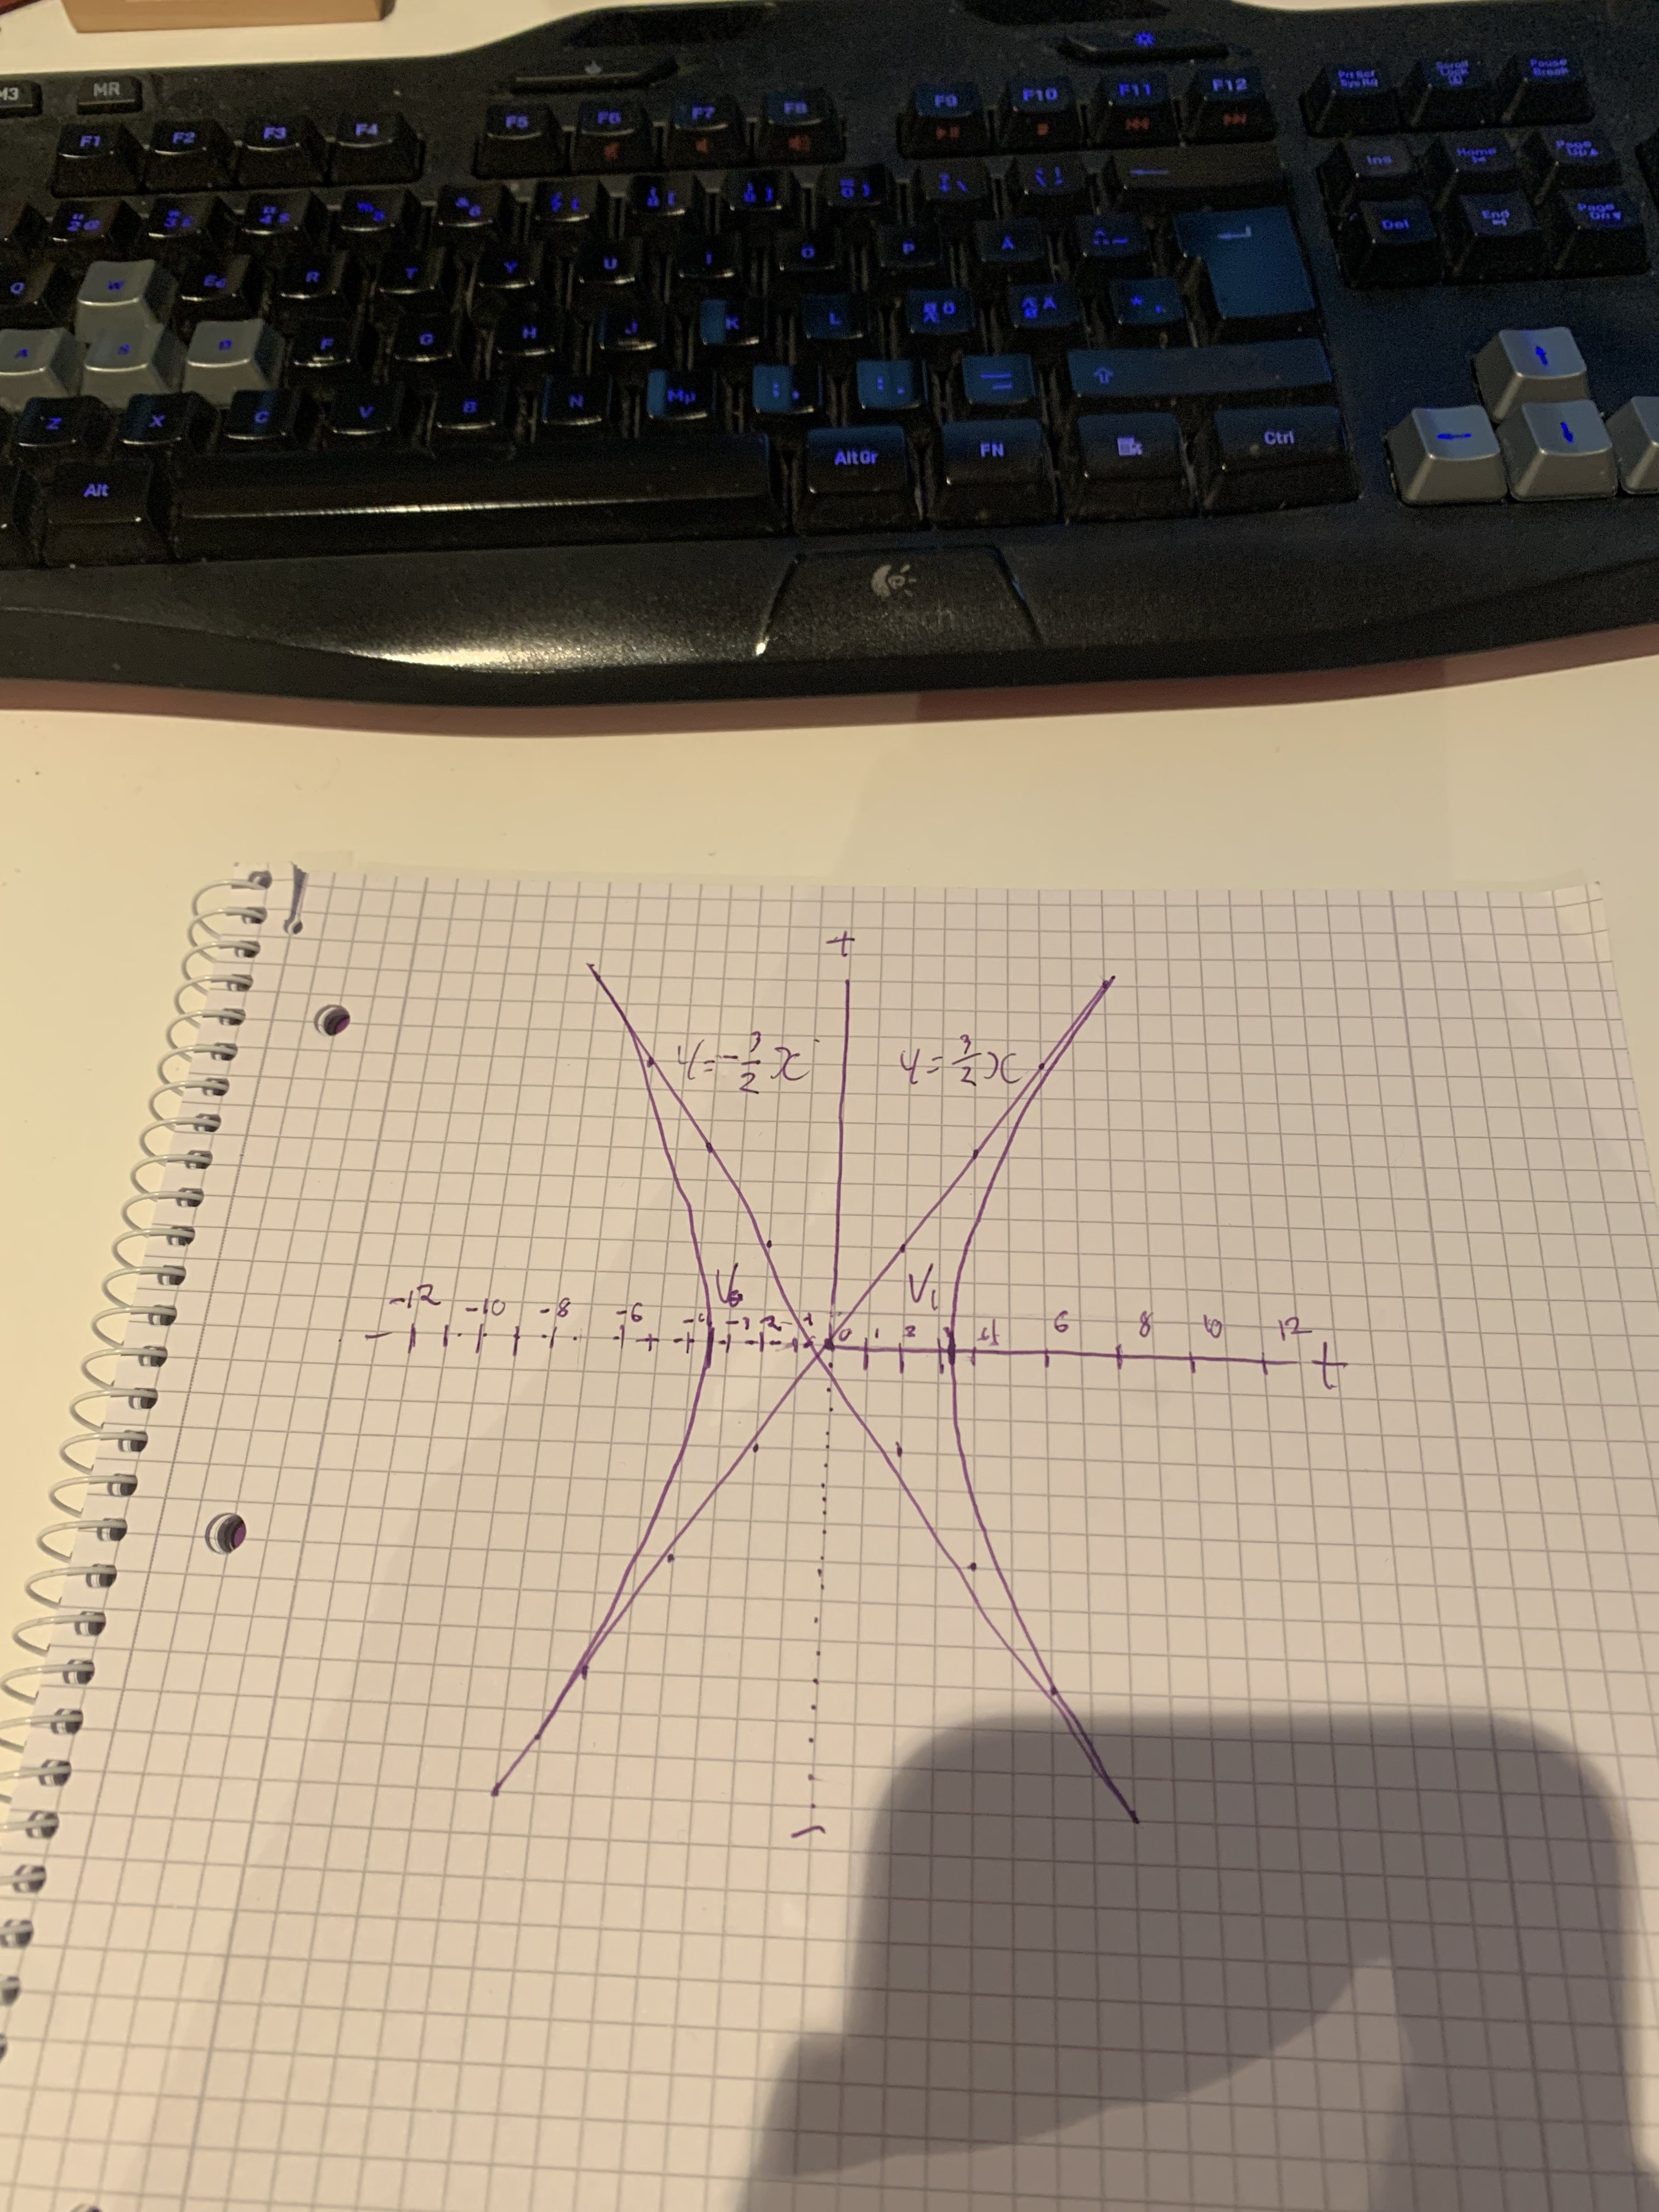
\includegraphics[trim={20cm 10cm 10cm 50cm},clip,width=.7\linewidth]{TMA01-T4-sketch}

		\caption{Sketch of conic}
		\label{fig:conic:sketch}
	\end{subfigure}%
	\begin{subfigure}{.5\textwidth}
		\centering
		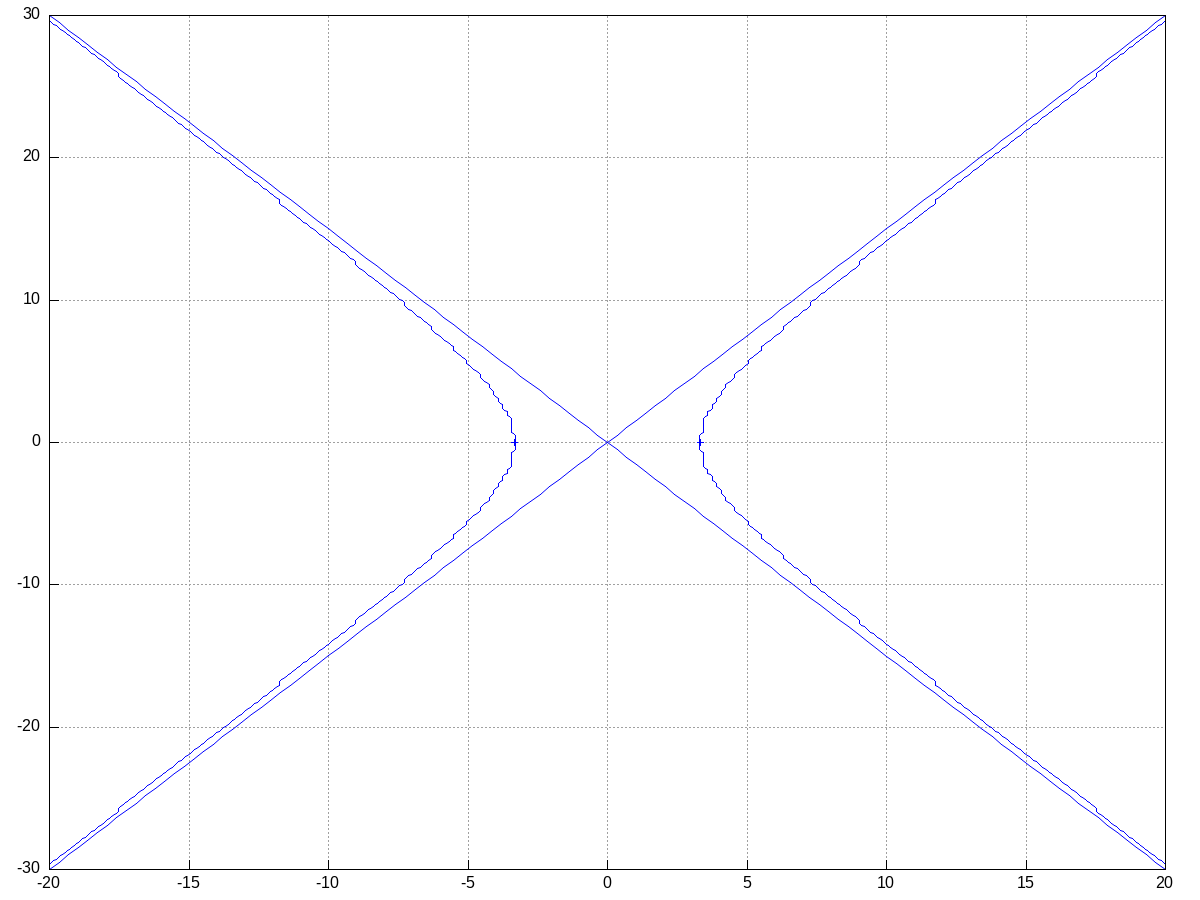
\includegraphics[width=.7\linewidth]{TMA01-T4}

		\caption{Maxima plot of conic}
		\label{fig:conic:maxima}
	\end{subfigure}

	\caption{Representations of conic}
	\label{fig:conic}
\end{figure}

\subsubsection{iii}

\begin{align*}
	 & \mathrm{eccentricity} & e               & = \frac {\sqrt {13}}2            \\
	 & \mathrm{foci}         & (\pm ae, 0)     & = (\pm\sqrt {13}~ \frac {5} 3,0) \\
	 & \mathrm{directrices}  & y = \pm\frac ae & = \pm \frac {20} {3\sqrt {13}}
\end{align*}

\subsubsection{iv}

$$
	\begin{pmatrix}
		x \\ y
	\end{pmatrix}
	=
	\begin{pmatrix}
		\frac {10}3\; \sec t \\
		5       \;\tan t     \\
	\end{pmatrix}
$$

To find the bounds we need to observe when we have the signs we want. Since we want a point with a negative $x$-sign and a possitive $y$-sign we need to see when the functions satasfy this.

$$\sec x < 0 \;\mathrm{if} -3\frac \pi 2 < x < - \frac \pi 2$$

and in the same interval we can see that

$$\tan x > 0 \;\mathrm{if} -\pi < x < - \frac \pi 2$$

Hence the interval for $t$ is $-\pi < t < - \frac \pi 2$.

\subsection{b}

$$6x^2 - 8xy + 5y^2 - 3x - 16y - 20 = 0$$

\subsubsection{i}

$$T = B^2 - 4 AC = 64 - 6 \times 5 = 34$$

Since $T > 0$ then the conic must be a Hyperbola.

\subsubsection{ii}

\begin{lstlisting}
	wxdraw2d(
        implicit(
            6 * x * x - 8 * x * y + 5 * y * y - 3 * x - 16 * y - 20 = 0,
            x,-10,10,
            y,-10,10
        )
	)$
\end{lstlisting}

\section{Question 5}

\subsection{a}

$$\mathrm A = (4 t + 2 , t - 1)$$

if $t=1$ then we get $(6,0)$. This means the entire line is translated up by $6$. If we then plug-in $t=2$ then we get $(10,1)$ which if we insert into the two point formula we get that the rise over run of this line is $\frac {10 - 6}{1 - 0} = 4$. This means the equation for the curve $\mathrm A$ traces is $y = 4x + 6$.

\subsection{b}

\begin{align*}
	\mid\vec{\mathrm{BA}}\mid          & =
	\begin {vmatrix}
	(4t + 2) - (2t + 5)                                     \\
	( t - 1) - (3t - 1)
	\end {vmatrix}                                          \\
	                                   & =
	\begin {vmatrix}
	2t - 3                                                  \\
	-2t
	\end {vmatrix}                                          \\
	                                   & =
	\sqrt {(2t - 3)^2 + (-2t)^2}                            \\
	                                   & =
	\sqrt {8t^2 -12t + 9}                                   \\
	\\
	d^2 ={\mid\vec{\mathrm{BA}}\mid}^2 & = 8 t^2 - 12 t + 9
\end{align*}

\section{c}

\begin{align}
	d^2 & = 8 t^2 - 12 t + 9                       \label{eq:l1}         \\
	    & = 8\Big(t^2 - \frac 32 t\Big) + 9                \label{eq:l2} \\
	    & = 8{\Big(t - \frac 34\Big)}^2 - \frac 9 {16} + 9 \label{eq:l3} \\
	    & = 8{\Big(t - \frac 34\Big)}^2 + \frac {135} {16} \label{eq:l4}
\end{align}
\begin{center}
	\parbox{7cm}{
		the minimum value of $d^2$ occurs when $t =\frac 34$.
		hence the minimum distance is $8.4 \mathrm m$ (to 2 s.f)}
\end{center}

The expression on (\ref{eq:l3}) ends up evaluating to
$$8(t^2 - \frac 32 t + \frac 9 {16}) - \frac 9{16} + 9 = 8t^2 - 12 t + \frac 9 {2} - \frac 9{16} + 9$$
which obviously is not equal to (\ref{eq:l2}).

Finally the statement that the distance is $\frac 32$ is incorrect since this is the square of the distance. The correct answer to the distance (including the compounded errir) is $\frac {\sqrt{135}}4$.

% (\ref{eq:l4}) then compounds the error from (\ref{eq:l3}). I do not believe this falls into the wording "[...] the working does not follow on from the previous line." yet it is a mistake.

Personally I would solve this task with a differentiation and a substutution but employing the same workings as the student we get as follows:

\begin{align}
	d^2 & = 8 t^2 - 12 t + 9                       \label{eq:2l1}         \\
	    & = 8\Big(t^2 - \frac 32 t\Big) + 9                \label{eq:2l2} \\
	    & = 8{\Big(t - \frac 34\Big)}^2 - \frac 92 + 9 \label{eq:2l3}     \\
	    & = 8{\Big(t - \frac 34\Big)}^2 + \frac 92 \label{eq:2l4}
\end{align}

\begin{center}
	\parbox{7cm}{
		The minimum value of $d^2$ occurs when $t =\frac 34$.
		hence the minimum distance is $\frac 3{\sqrt 2} \mathrm m = 2.12\mathrm m $ (to 2 s.f)}
\end{center}

\section{Question 6}

\subsection{a}

We can see the force diagram as Figure \ref{fig:fd}. This represents a simplification of the forces; angles nor magnatures are correct.

\begin{figure}[H]
	\centering
	\begin{tikzpicture}
		\coordinate (t1) at (2,   1.5);
		\coordinate (f)  at (-2,  -.5);
		\coordinate (fi) at (2,   .5);
		\coordinate (x)  at (.5,   -2);
		\coordinate (g)  at (0,   -3);
		\coordinate (n)  at (-0.5, 2);

		\coordinate (o)  at (0,    0);

		\coordinate (i)  at (6,    .25);
		\coordinate (j)  at (4.75, 1);
		\coordinate (ij) at (5,    0);

		\coordinate (o2) at (10,   0);
		\coordinate (t2) at (10,   2);
		\coordinate (g2) at (10,  -2);


		\draw (x) [dashed]-- (o);

		\draw (t1) node [above] {$T_1$};
		\draw (t1) [<-]-- (o);
		\draw (fi) [dashed]-- (o);

		\draw (f) node [above] {$F$};
		\draw (f) [<-]-- (o);

		\draw (g) [<-]-- (o);
		\draw (g) node [left] {$G_1$};

		\draw (n) [<-]-- (o);
		\draw (n) node [left] {$N$};

		\draw [fill] (o) circle [radius=0.1];

		\draw pic["$10^{\circ}$", draw=black, <->, angle eccentricity=1.3, angle radius=1cm]
			{angle=fi--o--t1};
		\draw pic["$20^{\circ}$", draw=black, <->, angle eccentricity=1.3, angle radius=2cm]
			{angle=g--o--x};

		\draw (i) [<-]--(ij);
		\draw (i) node [above] {$i$};

		\draw (j) [<-]--(ij);
		\draw (j) node [above] {$j$};

		\draw (t2) node [above] {$T_2$};
		\draw (t2) [<-]-- (o2);

		\draw (g2) [<-]-- (o2);
		\draw (g2) node [left] {$G_2$};

		\draw [fill] (o2) circle [radius=0.1];
	\end{tikzpicture}

	\caption{Force diagram}
	\label{fig:fd}
\end{figure}

\subsection{b}
\label{sec:newtonpain}

\begin{align*}
	\mathbf F + \mathbf N + \mathbf {T} + \mathbf G                                                          & = 0 \\
	-i~F + j~N + (i\cos {10^{\circ}}, j\sin {10^{\circ}})~T+ (-i\sin {20^{\circ}} -j\cos {20^{\circ}})~G     & = 0 \\
	-i~\mu N + j~N + (i\cos {10^{\circ}}, j\sin {10^{\circ}})~T+ (-i\sin {20^{\circ}} -j\cos {20^{\circ}})~G & = 0 \\
\end{align*}

NOTE: $\mid\mathbf X\mid = X$ and in this case for simplicity $T=T_1$ and $G = G_1$.

So if we split the equation into equations of its components we get:

\begin{align}
	\label{eq:subtarget}-\mu N + \cos {10^{\circ}} T- \sin {20^{\circ}} G & = 0 & N + T\sin {10^{\circ}} - G\cos {20^{\circ}} & = 0 \\
	                                                                      &     & - T\sin {10^\circ} + G \cos {20^\circ}      & = N
\end{align}

We can now substitute $N$ into the first equasion of (\ref{eq:subtarget}) getting

\begin{align*}
	-\mu N + \cos {10^{\circ}} T- \sin {20^{\circ}} G                                        & = 0 \\
	-\mu (- T\sin {10^\circ} + G \cos {20^\circ}) + \cos {10^{\circ}} T- \sin {20^{\circ}} G & = 0 \\
	T(\mu\sin {10^\circ} + \cos {10^\circ}) -G(\mu \cos {20^\circ} + \sin {20^{\circ}})      & = 0 \\
\end{align*}

Finally we can now get an expression for $T_1$.

\begin{align*}
	T_1 & = \frac {G(\mu \cos {20^\circ} + \sin {20^{\circ}})}{\mu\sin {10^\circ} + \cos {10^\circ}}           \\
	    & = \frac {17\times9.8(\mu \cos {20^\circ} + \sin {20^{\circ}})}{\mu\sin {10^\circ} + \cos {10^\circ}} \\
	    & \approx 17 \times 9.8 \times 0.5281                                                                  \\
	    & \approx 88 \mathrm N
\end{align*}

NOTE this answer is to two sigfigs.

\subsection{c}

Stemming for the fact that

$$T_2 - G_2 0 \iff T_2 = G_2$$

we know that

$$T_1 = T_2 = G_2 = mg$$

then we can use the answer from \ref{sec:newtonpain} to state that the mass of ball is

$$\frac {88}{9.8} \approx 9.0\mathrm{kg}$$

\end{document}

\begin{figure}[H]
	\centering
	\begin{tabular}{|c|c|c|}
		\hline
		Question & Status  & On attempt \\
		\hline
		Q1       & Correct & 1          \\
		Q2       & Correct & 2          \\
		Q3       & Correct & 1          \\
		Q4       & Correct & 3          \\

		\hline
	\end{tabular}
\end{figure}

\end{document}
